% tikzpic.tex
\documentclass[crop,tikz]{standalone}% 'crop' is the default for v1.0, before it was 'preview'

\usetikzlibrary{arrows,decorations.pathmorphing,decorations.pathreplacing,backgrounds,positioning,fit,matrix}
\usetikzlibrary{shapes,calc,patterns,arrows.meta}
\tikzset{
	vert/.style={circle,inner sep=1.5,fill=white,draw,minimum size=.3cm},
	edge/.style={color=black, thick},
	diredge/.style={->,>={Stealth[width=8pt,length=8pt]},color=black, thick},
	timelabel/.style={fill=white,font=\footnotesize, text centered},
	wave/.style={decorate,decoration={coil,aspect=0}},
	dirwave/.style={->, >={Stealth[width=8pt,length=8pt]},decorate,decoration={coil,aspect=0}},
	diredge2/.style={->,>={Stealth[width=8pt,length=8pt]}}
}
\begin{document}
	
	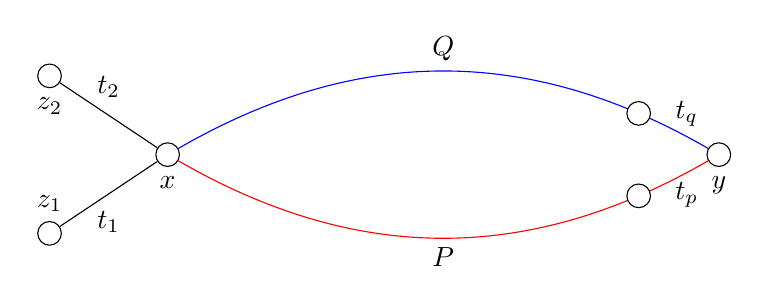
\begin{tikzpicture}
		
		\node [vert,label=below:$x$] (x) at (0, 0) {};
		\node [vert,label=below:$z_2$] (z2) at (-1.5, 1) {};
		\node [vert,label=above:$z_1$] (z1) at (-1.5, -1) {};
		\node [vert,label=below:$y$] (y) at (7, 0) {};
		
		\draw (z1) edge[] node[below, yshift=-1mm, text=black] {$t_1$}  (x);
		\draw (z2) edge[] node[above, yshift= 1mm,  text=black] {$t_2$} (x);
		\draw [red]
		(x) edge[] [bend right] node[below, text=black] {$P$} 
		node[vert, pos=0.87, color=black, fill=white] {}
		node[pos=0.96,below, text=black] {$t_p$} (y) ;
		\draw [blue]
		(x) edge[] [bend left] node[above, text=black] {$Q$} 
		node[vert, pos=0.87, color=black, fill=white] {}
		node[pos=0.96,above, text=black] {$t_q$}
		(y) ;
		
	\end{tikzpicture}
	
	
\end{document}